\chapter{introdução}

\section{Inserir figuras}

\begin{figure}[htb]
  \caption{\label{fig:teste} Figura de teste}
  \centering
  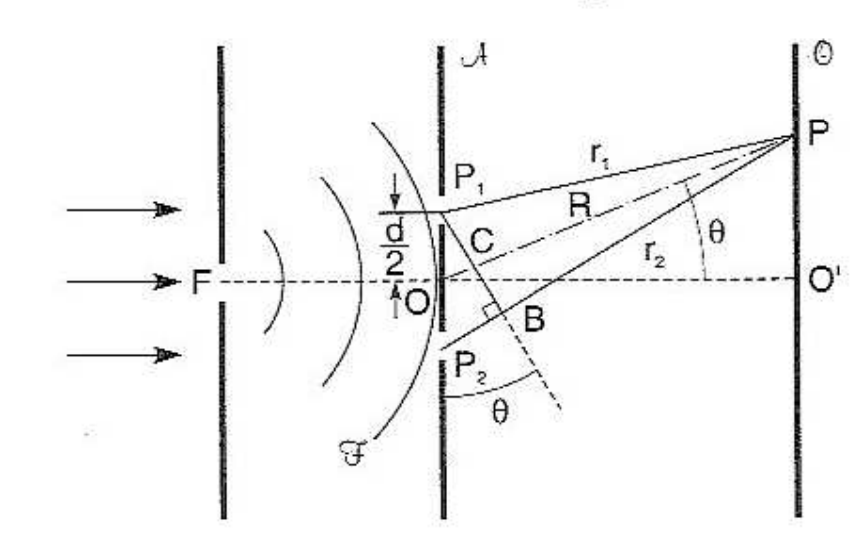
\includegraphics[width=0.8\textwidth]{images/teste.png}
  \fonte{Bota a fonte aqui}
\end{figure}

\section{Lista de Siglas}
Importante definir as siglas em main.tex  na seção "Declaração de Siglas" da seguinte forma:

%\siglalista{SIGLAS}{Significado da sigla}

Quando for fazer menção a sigla, basta usar \gls{SIGLAS}

\section{Coisas úteis}

\emph{Text} Para referenciar a termos estrangeuris (coisas que geralmente colocaria em itálico) \cite{moyses2}
\nocite{halliday4}

Para equações, tabelas e figuras, \autoref{fig:teste} e para nota de rodapé \footnote{É isso ai}



